\documentclass{article}\usepackage[]{graphicx}\usepackage[]{xcolor}
% maxwidth is the original width if it is less than linewidth
% otherwise use linewidth (to make sure the graphics do not exceed the margin)
\makeatletter
\def\maxwidth{ %
  \ifdim\Gin@nat@width>\linewidth
    \linewidth
  \else
    \Gin@nat@width
  \fi
}
\makeatother

\definecolor{fgcolor}{rgb}{0.345, 0.345, 0.345}
\newcommand{\hlnum}[1]{\textcolor[rgb]{0.686,0.059,0.569}{#1}}%
\newcommand{\hlstr}[1]{\textcolor[rgb]{0.192,0.494,0.8}{#1}}%
\newcommand{\hlcom}[1]{\textcolor[rgb]{0.678,0.584,0.686}{\textit{#1}}}%
\newcommand{\hlopt}[1]{\textcolor[rgb]{0,0,0}{#1}}%
\newcommand{\hlstd}[1]{\textcolor[rgb]{0.345,0.345,0.345}{#1}}%
\newcommand{\hlkwa}[1]{\textcolor[rgb]{0.161,0.373,0.58}{\textbf{#1}}}%
\newcommand{\hlkwb}[1]{\textcolor[rgb]{0.69,0.353,0.396}{#1}}%
\newcommand{\hlkwc}[1]{\textcolor[rgb]{0.333,0.667,0.333}{#1}}%
\newcommand{\hlkwd}[1]{\textcolor[rgb]{0.737,0.353,0.396}{\textbf{#1}}}%
\let\hlipl\hlkwb

\usepackage{framed}
\makeatletter
\newenvironment{kframe}{%
 \def\at@end@of@kframe{}%
 \ifinner\ifhmode%
  \def\at@end@of@kframe{\end{minipage}}%
  \begin{minipage}{\columnwidth}%
 \fi\fi%
 \def\FrameCommand##1{\hskip\@totalleftmargin \hskip-\fboxsep
 \colorbox{shadecolor}{##1}\hskip-\fboxsep
     % There is no \\@totalrightmargin, so:
     \hskip-\linewidth \hskip-\@totalleftmargin \hskip\columnwidth}%
 \MakeFramed {\advance\hsize-\width
   \@totalleftmargin\z@ \linewidth\hsize
   \@setminipage}}%
 {\par\unskip\endMakeFramed%
 \at@end@of@kframe}
\makeatother

\definecolor{shadecolor}{rgb}{.97, .97, .97}
\definecolor{messagecolor}{rgb}{0, 0, 0}
\definecolor{warningcolor}{rgb}{1, 0, 1}
\definecolor{errorcolor}{rgb}{1, 0, 0}
\newenvironment{knitrout}{}{} % an empty environment to be redefined in TeX

\usepackage{alltt}
\usepackage{hyperref}
\usepackage{blindtext}
\usepackage{graphicx}
\usepackage[a4paper, total={6in, 8in}]{geometry}
\IfFileExists{upquote.sty}{\usepackage{upquote}}{}
\begin{document}



\section{Chapter 3. Modern Methods of Data Visualisation}

\section{Chapter 3.1 Introduction to Modern Data Visualization Methods}
As data grows increasingly complex and vast, the tools and techniques for effectively conveying this information continue to expand and refine. This chapter tackles the modern data visualization methods, offering a comprehensive exploration of various visualization techniques, along with tangible examples accompanied by their underlying code.

\subsection{3.3.2 Data Sets}
\begin{enumerate}
\item Mtcars dataset: The mtcars dataset in R is a built-in dataset that contains information about various car models. It provides data on the characteristics of 32 different car models, which were available in the early 1970s. The dataset includes a total of 11 variables, each representing different attributes of these cars, such as miles per gallon (mpg), horsepower (hp), number of cylinders (cyl), and more. The mtcars dataset is often used for data analysis, visualization, and statistical modeling, making it a useful resource for exploring and practicing data science techniques in R.
\end{enumerate}

\section{Chapter 3.2 Scatter Plots and Bubble Charts}
Scatter plots and bubble charts are fundamental data visualization techniques that provide valuable insights into the relationships and patterns within datasets. These visualizations are particularly effective for representing data points, making comparisons, and revealing trends.

\subsection{3.2.1 Scatter Plots}
Dot plots, also known as dot charts or dot density plots, offer a straightforward yet mathematically intriguing method for visualizing data. At their core, dot plots display individual data points as dots along a single axis, with each dot representing a single observation. The mathematical interest of dot plots lies in their ability to provide a simple visual representation of data distribution, center, and spread. While they don't rely on complex equations or statistical principles, dot plots make it easy to observe important characteristics of data, such as the mode (the most frequent value), skewness (asymmetry), and potential outliers. They're particularly useful for comparing multiple data sets, identifying patterns, and detecting data irregularities, all while offering an intuitive and accessible way to grasp the fundamental concepts of data visualization and data analysis. This simplicity is what makes dot plots a valuable tool for both introductory statistics education and exploratory data analysis.

\subsection{Scatter Plots in Practice}
In this example, we'll create a scatter plot that visualizes the relationship between two variables - the weight of cars and the amount of miles traveled per gallon of petrol. We'll use the "mtcars" R dataset.

\begin{knitrout}
\definecolor{shadecolor}{rgb}{0.969, 0.969, 0.969}\color{fgcolor}\begin{kframe}


{\ttfamily\noindent\itshape\color{messagecolor}{\#\# `geom\_smooth()` using formula = 'y \textasciitilde{} x'}}\end{kframe}
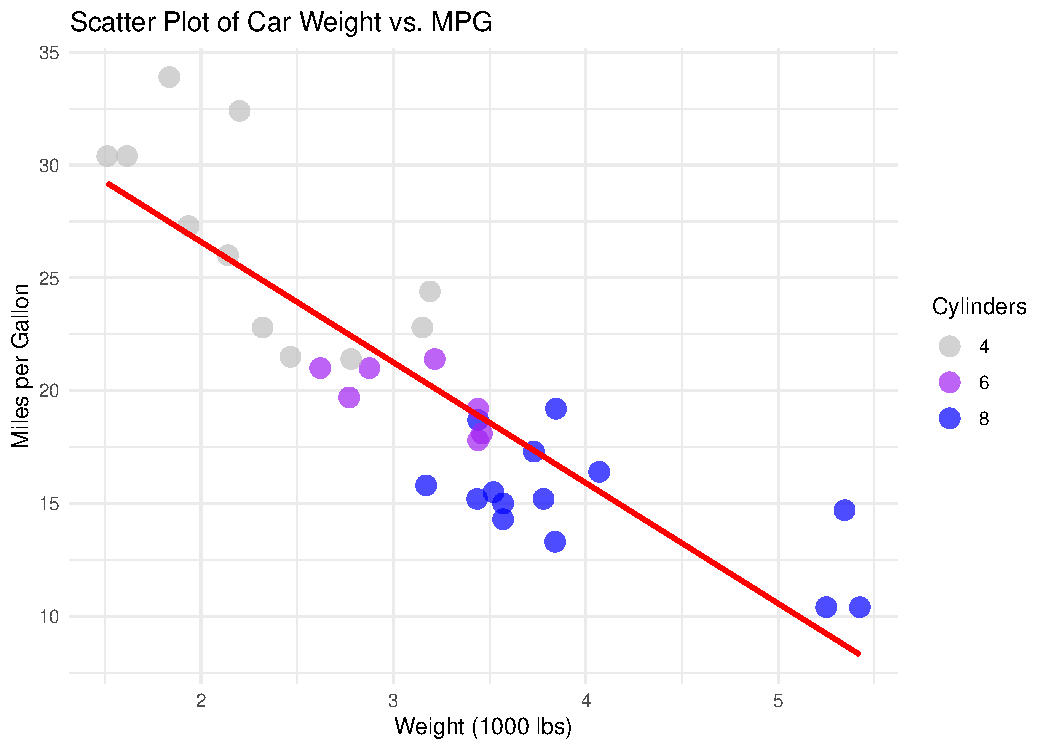
\includegraphics[width=\maxwidth]{figure/scatter-plot-chunk-1} 
\end{knitrout}

\subsection{Analysis}
The scatter plot displays the relationship between car weight (in thousands of pounds, "wt") and fuel efficiency (miles per gallon, "mpg") for different car models. While this graph plots two variable, through the use of colour, additional lines, and other subtle details, we can make of this basic graph, a more readable and visually interesting figure which the reader can get easily gather information from. Here are the key characteristics of the plot:
\begin{itemize}
    \item Color-Coded Cylinders: The points are color-coded based on the number of cylinders in the engine (4, 6, and 8 cylinders). This allows for a quick visual differentiation of car types, enhancing the understanding of the data.
    \item Point Size and Transparency: Points have been enlarged and have a subtle degree of transparency for visual appeal. Larger, more prominent points are easier to see, while transparency helps in the visualization of overlapping points.
    \item Linear Regression Line: A red linear regression trend line is included. It provides a visual representation of the overall relationship between car weight and fuel efficiency, indicating a negative correlation—cars tend to have lower fuel efficiency as their weight increases.\\
\end{itemize}

\subsection{Regression and the Regression Line}
\textbf{Regression} is a statistical technique used to model and understand the relationship between two or more variables. It is a fundamental tool in data analysis and predictive modeling. In simple linear regression, a linear equation is used to describe the relationship between a dependent variable (the one you want to predict) and one or more independent variables (the predictors).The equation takes the form of \(Y = aX + b\), where \(Y\) is the dependent variable, \(X\) is the independent variable, \(a\) is the slope, and \(b\) is the intercept.\\
Regression analysis calculates the best-fit line that minimizes the sum of squared differences between the predicted and actual values. This line provides valuable insights into the strength and direction of the relationship between variables, allowing us to make predictions and understand how changes in one variable affect another. Adding regression lines to scatter plots can enhance their value by providing a clearer depiction of trends and enabling more accurate predictions, turning the plot into a predictive tool rather than just a visual representation of data points.


\subsection{3.2.2 Bubble Charts}
Bubble charts, like scatter plots, are a valuable tool in data visualization that represent data points as bubbles or circles on a two-dimensional plane. They introduce an additional dimension by encoding data using the size of these bubbles. The mathematical intricacies behind bubble charts involve principles of geometry and data scaling.\\
To calculate the size of each bubble, a scaling factor is applied to map the data values to a suitable range for bubble sizes. Typically, linear or nonlinear scaling methods are used to ensure that the bubble sizes accurately reflect the underlying data. The equations used in bubble charts are relatively straightforward, but the challenge lies in selecting appropriate scaling methods and ensuring that the size variations effectively convey the data's significance. 

\subsubsection{Advantages}
\begin{itemize}
    \item Visualising three data attributes in a single chart.
    \item Effective for exploring complex relationships and identifying patterns. 
\end{itemize}

\subsection{Bubble Charts in Practice}
 This bubble plot visualizes data from the same dataset as above. The purpose of this plot is to depict the relationship between car models and their fuel efficiency (mpg) while using the size of the bubbles to represent the car's horsepower (hp) and color-coding the bubbles based on the number of cylinders (cyl).

\begin{knitrout}
\definecolor{shadecolor}{rgb}{0.969, 0.969, 0.969}\color{fgcolor}
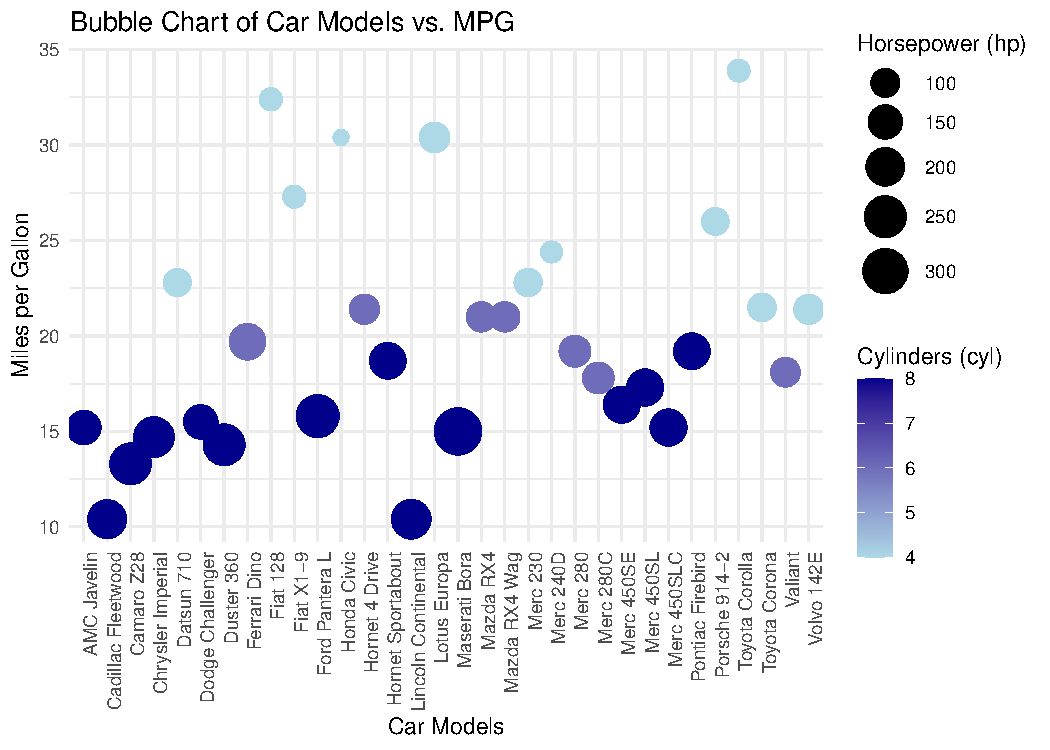
\includegraphics[width=\maxwidth]{figure/buble-plot-chunk-1} 
\end{knitrout}

\section{Analysis}
The plot's title, axis labels, and legends provide context and clarity to the visualization, making it accessible and informative. Additionally, the choice of a gradient color scale for the number of cylinders enhances the visual appeal and aids in interpreting the data.This bubble plot allows for quick comparisons between multiple characteristics of different car models.The resulting bubble plot effectively conveys several key insights:
\begin{enumerate}
\item \textbf{Car Model vs. MPG}: The x-axis displays the car models, offering a clear representation of each vehicle in the dataset. The bubble plot is particularly useful for displaying nominal data, such as car model names, as it allows easy identification and comparison.
\item \textbf{Miles per Gallon (MPG)}: The y-axis measures miles per gallon, representing the fuel efficiency of each car model. Higher bubbles indicate better fuel efficiency. This variable, which is continuous, is positioned vertically to demonstrate how each car model's fuel efficiency relates to others.
\item \textbf{Horsepower (HP)}: The size of each bubble represents the car's horsepower (hp). Larger bubbles correspond to higher horsepower, providing an additional dimension to the data. The size encoding helps identify more powerful cars.
\item \textbf{Cylinders (Cyl)}: The color of each bubble is determined by the number of cylinders (cyl) in the car's engine. The color scheme adds a categorical aspect to the visualization, making it easy to differentiate between cars with different cylinder counts.
\end{enumerate}


\section*{Chapter 3.3 Bar Charts and Histograms}
\subsection*{Bar Charts}
A bar chart is a very important method to present data. It organizes information into vertical bars.  Bar charts have lots of advantages in data visualization. It can present data categories in a frequency distribution. A bar chart is best for comparing classified data. Especially when the values are close, because the human perception of height is better than other visual elements (such as area, angle, etc.), the use of a bar chart is more appropriate. These bars usually have different lengths, and every length is proportional to the size of the information they present.\\
R uses the function $barplot()$ to create bar charts. R can draw both vertical and Horizontal bars in the bar chart. In the bar chart, each of the bars can be given different colors.\\
R is a programming language for data analysis and statistical computing, and its advent has made data visualization more straightforward and accessible. Among the various tools available in R, ggplot2 stands out as one of the most renowned and powerful tools for creating data visualizations. It offers a wealth of data visualization capabilities and is celebrated for its versatility and aesthetic appeal. In this chapter, we will focus on how to use ggplot2 to create bar charts for data visualization.\\

\subsection*{3.3.1 Different Types of Bar Charts}
Here is an overview of the different types of bar charts. \\
\paragraph{Vertical Bar Chart}
This is the most common bar chart. We use different vertical columns to display and compare the values of different categories in the same dimension, where the X-axis represents the contrasting categories and the Y-axis represents the frequency or count of their categories.\\
\paragraph{Horizontal Bar Chart}
This is very similar to a vertical bar chart but rotated 90 degrees. Categories are shown on the y-axis and frequency or count are shown on the x-axis. Horizontal bar charts are especially useful when category names are long or when there are numerous categories.
\paragraph{Multi-set Bar Chart}
Also known as a grouped bar chart or clustered bar chart. A multi-set bar chart is used to represent and compare different sub-groups within individual categories. This type of chart is useful when you want to show and compare multiple sets of data side-by-side.
Multi-set Bar charts can be horizontal or vertical like the other normal bar charts, and the length of each bar represents the frequency or count of their categories.
\paragraph{Stacked bar chart}
Similar to bar charts, stacked bar charts are often used to compare different classes of values and, within each class of values, are divided into sub-classes, which are often referred to by different colors. Each segment's size is proportional to the frequency or count that it represents from the sub-category. The entire bar's length represents the cumulative total of all the sub-categories.
However, it is very easy to get confused when there are too many categories.

\subsection*{3.3.2 Advantages of Bar Charts}
\begin{enumerate}
\item \textbf{Clarity and Simplicity}: Bar charts are structurally simple, making them easy to read and understand, allowing audiences to quickly grasp key information.
    \item \textbf{Effective Comparison}: They provide a visual representation that makes comparing the size or value of different categories straightforward, especially when comparing a limited number of categorical data.
    \item \textbf{High Flexibility}: They can be used to represent any type of data, be it continuous or discrete.
    \item \textbf{Multilevel Representation}: Stacked or grouped bar charts can be used to represent multiple data series.
\end{enumerate}

\subsection*{3.3.3 Disadvantages of Bar Charts}
\begin{enumerate}
    \item \textbf{Limited Data Representation}: They might not be suitable for representing large datasets as things can get cluttered.
    \item \textbf{Potential Misinterpretation}: Without a zero baseline, bar charts can be misleading as they might exaggerate differences.
    \item \textbf{Overcomplexity with Many Categories}: If there are too many bars, it can be challenging to discern information effectively.
    \item \textbf{Requires Categorical Data}: Bar charts are not ideal for representing trends over continuous data, where line graphs might be more appropriate.
\end{enumerate}

In this section, I will analyze the air quality dataset provided by the United States Environmental Protection Agency. In our dataset, we have data from over 200 locations. The Air Quality Index (AQI) ranges from 0 to 500. A higher AQI indicates increased levels of air pollution, leading to heightened health concerns. This implies that as the AQI rises, there is a greater risk to public health.

\begin{knitrout}
\definecolor{shadecolor}{rgb}{0.969, 0.969, 0.969}\color{fgcolor}\begin{kframe}
\begin{alltt}
\hlstd{data} \hlkwb{<-} \hlkwd{read.csv}\hlstd{(}\hlstr{"c4_epa_air_quality.csv"}\hlstd{)}
\hlkwd{ggplot}\hlstd{(data,} \hlkwd{aes}\hlstd{(}\hlkwc{x} \hlstd{= aqi))} \hlopt{+}
  \hlkwd{geom_bar}\hlstd{()} \hlopt{+}
  \hlkwd{labs}\hlstd{(}\hlkwc{title} \hlstd{=} \hlstr{"Bar Chart Example 1"}\hlstd{,} \hlkwc{x} \hlstd{=}
         \hlstr{"Air Quality Index/units"}\hlstd{,} \hlkwc{y} \hlstd{=} \hlstr{"number/sites"}\hlstd{)} \hlopt{+}
  \hlkwd{theme_minimal}\hlstd{()}
\end{alltt}
\end{kframe}
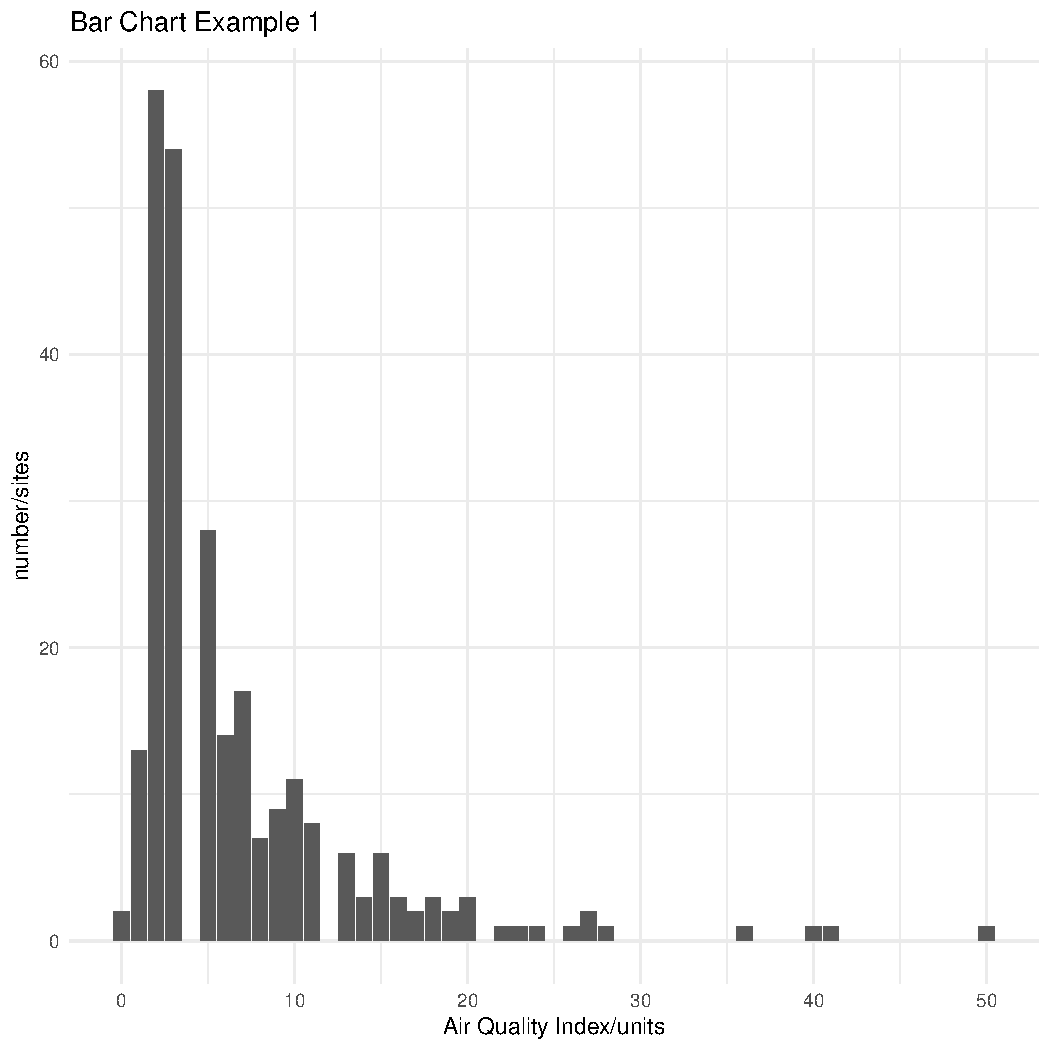
\includegraphics[width=\maxwidth]{figure/my_plot1-1} 
\end{knitrout}

The above code is not optimal. Upon examinationan, we can see that there is an excussive number of different categories on the x-axis. Consequently, the multitude of vertical bars in the graph can potentially overwhelm and confuse readers. 
In order to solve the problem, we can use the “cut” function to divide the data into intervals of five units each. For instance, values from 0-5 would constitute one group, 6-10 another, 11-15 would form the next group, and so forth.


\begin{knitrout}
\definecolor{shadecolor}{rgb}{0.969, 0.969, 0.969}\color{fgcolor}\begin{kframe}
\begin{alltt}
\hlstd{data} \hlkwb{<-} \hlkwd{read.csv}\hlstd{(}\hlstr{"c4_epa_air_quality.csv"}\hlstd{)} \hlcom{#}
\hlcom{# load ggplot2 package}
\hlkwd{library}\hlstd{(ggplot2)}

\hlcom{# Use the cut function to divide the data into groups of five intervals}
\hlstd{data}\hlopt{$}\hlstd{group} \hlkwb{<-} \hlkwd{cut}\hlstd{(data}\hlopt{$}\hlstd{aqi,} \hlkwc{breaks} \hlstd{=}
                    \hlkwd{seq}\hlstd{(}\hlnum{0}\hlstd{,} \hlkwd{max}\hlstd{(data}\hlopt{$}\hlstd{aqi)} \hlopt{+} \hlnum{5}\hlstd{,} \hlkwc{by} \hlstd{=} \hlnum{5}\hlstd{),}
                  \hlkwc{right} \hlstd{=} \hlnum{FALSE}\hlstd{,} \hlkwc{include.lowest} \hlstd{=} \hlnum{TRUE}\hlstd{)}
\hlstd{data}\hlopt{$}\hlstd{group} \hlkwb{<-} \hlkwd{as.numeric}\hlstd{(data}\hlopt{$}\hlstd{group)}

\hlcom{# Y-axis representing the number of occurrences of the X-axis label in the data}
\hlkwd{ggplot}\hlstd{(data,} \hlkwd{aes}\hlstd{(}\hlkwc{x} \hlstd{= group))} \hlopt{+}
  \hlkwd{geom_bar}\hlstd{()} \hlopt{+}
  \hlkwd{labs}\hlstd{(}\hlkwc{title} \hlstd{=} \hlstr{"Bar Chart Example 1"}\hlstd{,}
       \hlkwc{x} \hlstd{=} \hlstr{"Air Quality Index/units"}\hlstd{,} \hlkwc{y} \hlstd{=} \hlstr{"Number/sites"}\hlstd{)} \hlopt{+}
  \hlkwd{theme_minimal}\hlstd{()} \hlopt{+}
  \hlkwd{scale_x_discrete}\hlstd{(}\hlkwc{labels} \hlstd{= scales}\hlopt{::}\hlkwd{label_number}\hlstd{(}\hlkwc{accuracy} \hlstd{=} \hlnum{5}\hlstd{))}
\end{alltt}
\end{kframe}
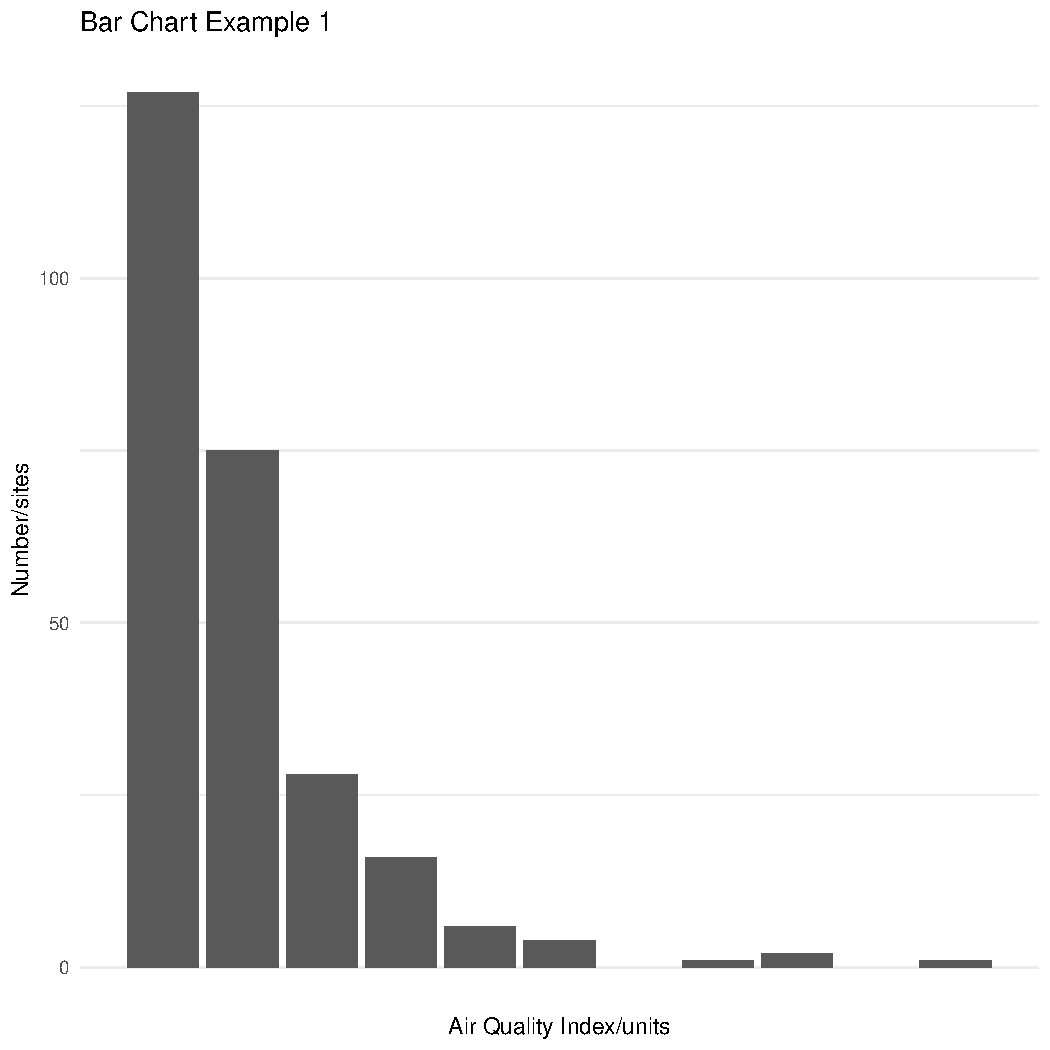
\includegraphics[width=\maxwidth]{figure/my_plot2-1} 
\end{knitrout}

We can also add some color to make our plot more attractive, here we can add sone color as well. In the code below, we set the color of the bar chart to blue while specifying the border color as black.

\begin{knitrout}
\definecolor{shadecolor}{rgb}{0.969, 0.969, 0.969}\color{fgcolor}\begin{kframe}
\begin{alltt}
\hlcom{# read CSV dater set}
\hlstd{data} \hlkwb{<-} \hlkwd{read.csv}\hlstd{(}\hlstr{"c4_epa_air_quality.csv"}\hlstd{)}

\hlcom{# load ggplot2 }
\hlkwd{library}\hlstd{(ggplot2)}

\hlcom{# Use the cut function to divide the data into groups of five intervals}
\hlstd{data}\hlopt{$}\hlstd{group} \hlkwb{<-} \hlkwd{cut}\hlstd{(data}\hlopt{$}\hlstd{aqi,} \hlkwc{breaks} \hlstd{=} \hlkwd{seq}\hlstd{(}\hlnum{0}\hlstd{,} \hlkwd{max}\hlstd{(data}\hlopt{$}\hlstd{aqi)} \hlopt{+} \hlnum{5}\hlstd{,} \hlkwc{by} \hlstd{=} \hlnum{5}\hlstd{),}
                  \hlkwc{right} \hlstd{=} \hlnum{FALSE}\hlstd{,} \hlkwc{include.lowest} \hlstd{=} \hlnum{TRUE}\hlstd{)}
\hlstd{data}\hlopt{$}\hlstd{group} \hlkwb{<-} \hlkwd{as.numeric}\hlstd{(data}\hlopt{$}\hlstd{group)}
\hlcom{# Converts the group column to numeric type}

\hlkwd{ggplot}\hlstd{(data,} \hlkwd{aes}\hlstd{(}\hlkwc{x} \hlstd{= group))} \hlopt{+}
  \hlkwd{geom_bar}\hlstd{(}\hlkwc{color}\hlstd{=}\hlstr{"black"}\hlstd{,}\hlkwc{fill}\hlstd{=}\hlstr{"blue"}\hlstd{)} \hlopt{+}
  \hlkwd{labs}\hlstd{(}\hlkwc{title} \hlstd{=} \hlstr{"Bar Chart Example 1"}\hlstd{,} \hlkwc{x} \hlstd{=} \hlstr{"Air Quality Index/units"}\hlstd{,}
       \hlkwc{y} \hlstd{=} \hlstr{"Number/sites"}\hlstd{)} \hlopt{+}
  \hlkwd{theme_minimal}\hlstd{()} \hlopt{+}
  \hlkwd{scale_x_discrete}\hlstd{(}\hlkwc{labels} \hlstd{= scales}\hlopt{::}\hlkwd{label_number}\hlstd{(}\hlkwc{accuracy} \hlstd{=} \hlnum{5}\hlstd{))}
\end{alltt}
\end{kframe}
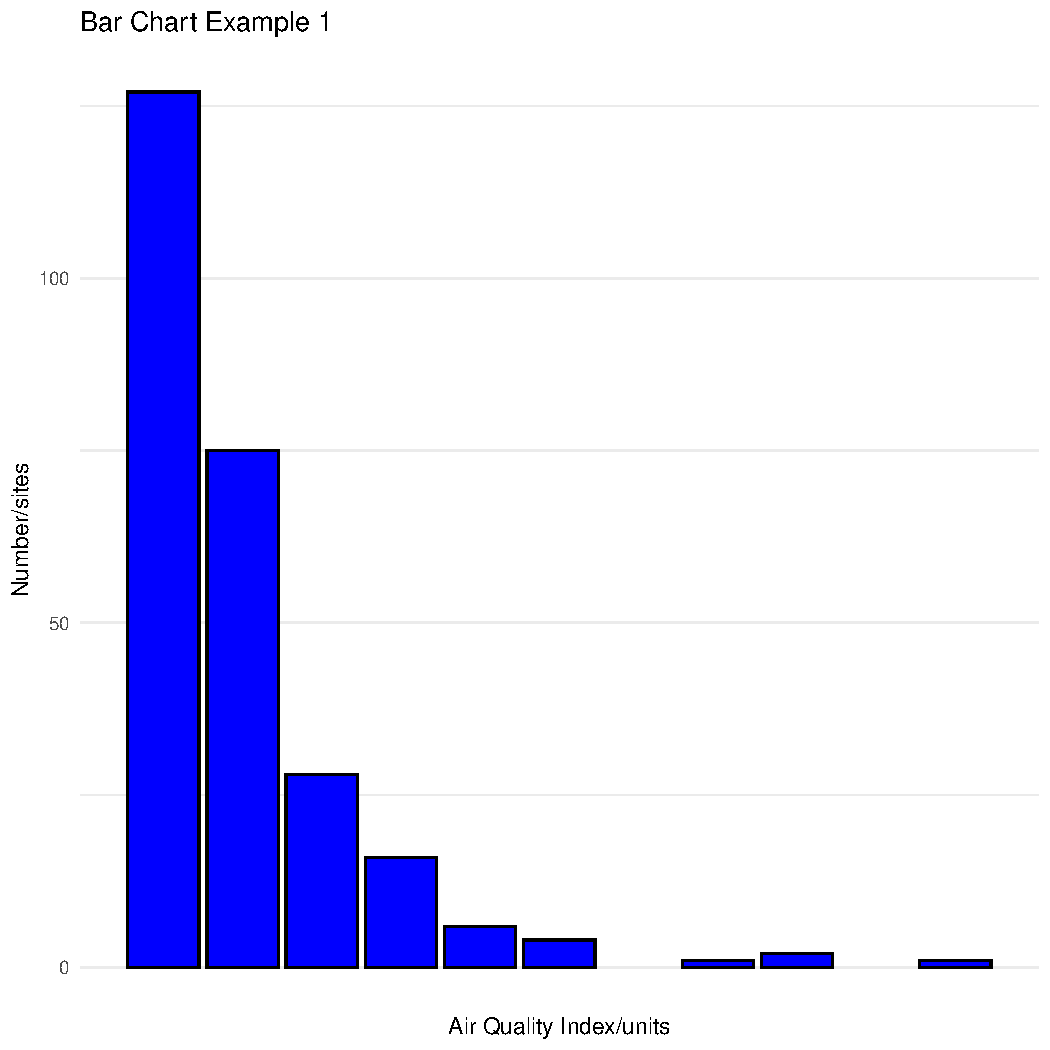
\includegraphics[width=\maxwidth]{figure/my_plot3-1} 
\end{knitrout}

Finally, we add lables to the X-axis to define the range of each categories.
\begin{knitrout}
\definecolor{shadecolor}{rgb}{0.969, 0.969, 0.969}\color{fgcolor}\begin{kframe}
\begin{alltt}
\hlcom{# read csv}
\hlstd{data} \hlkwb{<-} \hlkwd{read.csv}\hlstd{(}\hlstr{"c4_epa_air_quality.csv"}\hlstd{)}

\hlcom{# load ggplot2}
\hlkwd{library}\hlstd{(ggplot2)}

\hlcom{# Use the cut function to divide the data into groups of five intervals}
\hlstd{breaks_list} \hlkwb{<-} \hlkwd{seq}\hlstd{(}\hlnum{0}\hlstd{,} \hlkwd{max}\hlstd{(data}\hlopt{$}\hlstd{aqi)} \hlopt{+} \hlnum{5}\hlstd{,} \hlkwc{by} \hlstd{=} \hlnum{5}\hlstd{)}
\hlstd{data}\hlopt{$}\hlstd{group} \hlkwb{<-} \hlkwd{cut}\hlstd{(data}\hlopt{$}\hlstd{aqi,} \hlkwc{breaks} \hlstd{= breaks_list,}
                  \hlkwc{right} \hlstd{=} \hlnum{FALSE}\hlstd{,} \hlkwc{include.lowest} \hlstd{=} \hlnum{TRUE}\hlstd{)}


\hlkwd{ggplot}\hlstd{(data,} \hlkwd{aes}\hlstd{(}\hlkwc{x} \hlstd{= group))} \hlopt{+}
  \hlkwd{geom_bar}\hlstd{(}\hlkwc{color}\hlstd{=}\hlstr{"black"}\hlstd{,} \hlkwc{fill}\hlstd{=}\hlstr{"blue"}\hlstd{)} \hlopt{+}
  \hlkwd{labs}\hlstd{(}\hlkwc{title} \hlstd{=} \hlstr{"Bar Chart Example 2"}\hlstd{,} \hlkwc{x} \hlstd{=} \hlstr{"Air Quality Index/units"}\hlstd{,}
       \hlkwc{y} \hlstd{=} \hlstr{"Number/sites"}\hlstd{)} \hlopt{+}
  \hlkwd{theme_minimal}\hlstd{()} \hlopt{+}
  \hlkwd{scale_x_discrete}\hlstd{(}\hlkwc{labels} \hlstd{=} \hlkwd{paste0}
                   \hlstd{(breaks_list[}\hlopt{-}\hlkwd{length}\hlstd{(breaks_list)],} \hlstr{"-"}\hlstd{, breaks_list[}\hlopt{-}\hlnum{1}\hlstd{]))}
\end{alltt}
\end{kframe}
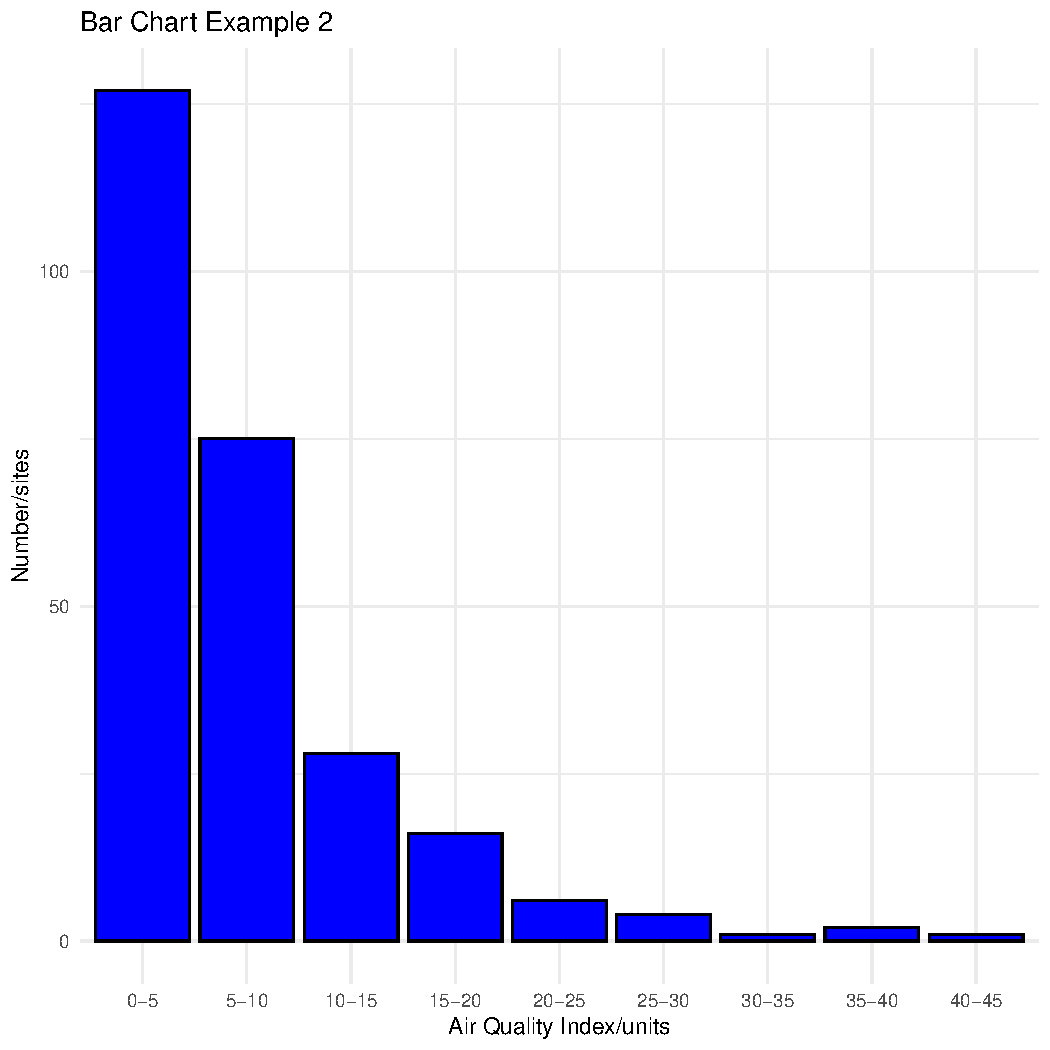
\includegraphics[width=\maxwidth]{figure/my_plot4-1} 
\end{knitrout}

\section{Chapter 3.4 Heatmaps and Tree Maps}
\\  
\\In this chapter, we explore two powerful data visualisation techniques: heatmaps and treemaps. These methods are instrumental for conveying intricate data structures and patterns, offering unique ways to represent multivariate information, making them indispensable tools for data scientists.
\\  
\\We will delve into the theory behind heatmaps and treemaps, understand how to create them using popular data visualization libraries, and demonstrate their practical applications with real-world examples. By the end of this chapter, you will be well-equipped to leverage heatmaps and treemaps to gain insights from complex and hierarchical datasets.

\subsection{3.4.1 Heatmaps - Fire in Brazil}
\\  
\\The heatmap is a data visualisation technique that uses color coding to represent different intensity.
\\  
\\In this illustrative example, heatmaps is used to visualize fire occurrences in Brazil. These heatmaps offer a spatially coherent representation, highlighting regions at high risk and seasonal patterns. Here, the heatmap is a power tool for identifying the risk of fire incidents. The data-driven insights empowers us to make informed decisions concerning preventive measures and strategies for firefighting.
\\  
\\All data obtain from \href{https://firms.modaps.eosdis.nasa.gov/}{NASA}. Each dataset from 2013 to 2022 contains more than 200,000 observations. Across the decade, there are over 3 million observations. The trend is impossible to analyze by eye. However, an exploratory analysis using heatmaps provides insights into this data.





\begin{knitrout}
\definecolor{shadecolor}{rgb}{0.969, 0.969, 0.969}\color{fgcolor}\begin{kframe}
\begin{alltt}
\hlcom{# Obtain the Brazil map data}
\hlstd{brazil_map} \hlkwb{<-} \hlkwd{map_data}\hlstd{(}\hlstr{"world"}\hlstd{,} \hlkwc{region} \hlstd{=} \hlstr{"Brazil"}\hlstd{)}

\hlcom{# Create the heatmap of fire occurrences}
\hlstd{fire_heatmap} \hlkwb{<-} \hlkwd{ggplot}\hlstd{(confident_fire_fy22,} \hlkwd{aes}\hlstd{(}\hlkwc{x} \hlstd{= longitude,} \hlkwc{y} \hlstd{= latitude))} \hlopt{+}
  \hlkwd{geom_polygon}\hlstd{(}\hlkwc{data} \hlstd{= brazil_map,} \hlkwd{aes}\hlstd{(}\hlkwc{x} \hlstd{= long,} \hlkwc{y} \hlstd{= lat,} \hlkwc{group} \hlstd{= group),}
               \hlkwc{fill} \hlstd{=} \hlstr{"#bdbdbd"}\hlstd{)} \hlopt{+}
  \hlkwd{geom_bin2d}\hlstd{(}\hlkwc{bins} \hlstd{=} \hlnum{300}\hlstd{)} \hlopt{+}
  \hlkwd{scale_fill_gradient}\hlstd{(}\hlkwc{low} \hlstd{=} \hlstr{"#fee6ce"}\hlstd{,} \hlkwc{high} \hlstd{=} \hlstr{"#d7301f"}\hlstd{)} \hlopt{+}
  \hlkwd{coord_fixed}\hlstd{(}\hlkwc{ratio} \hlstd{=} \hlnum{1}\hlstd{)} \hlopt{+}
  \hlkwd{theme_minimal}\hlstd{()}\hlopt{+}
  \hlkwd{theme}\hlstd{(}\hlkwc{axis.text} \hlstd{=} \hlkwd{element_text}\hlstd{(}\hlkwc{size} \hlstd{=} \hlnum{10}\hlstd{))}

\hlkwd{print}\hlstd{(fire_heatmap)}
\end{alltt}
\end{kframe}\begin{figure}
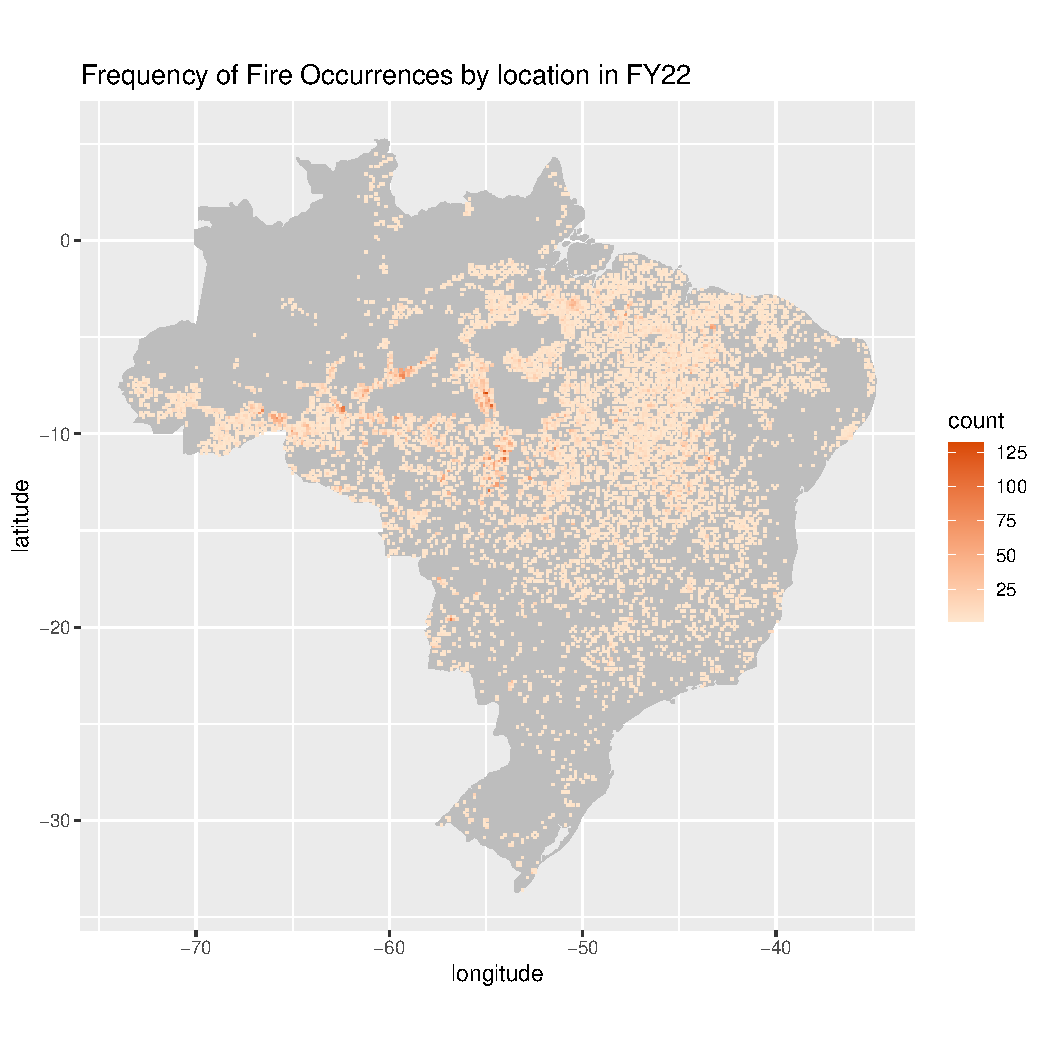
\includegraphics[width=\maxwidth]{figure/fire-by-location-fy22-1} \caption[Frequency of Fire Occurrences by location in FY22]{Frequency of Fire Occurrences by location in FY22}\label{fig:fire-by-location-fy22}
\end{figure}

\end{knitrout}
\\From the heatmap, we can observe that certain locations have significantly higher fires count. However, we do not know the cause of this. Is this due to geographical location, or is it because fires were mostly man-made and used to clear forest areas for agriculture use?
\\  
\\Colour selection from \href{https://colorbrewer2.org/#type=sequential&scheme=Oranges&n=9}{colorbrewer2}.



\begin{knitrout}
\definecolor{shadecolor}{rgb}{0.969, 0.969, 0.969}\color{fgcolor}\begin{kframe}
\begin{alltt}
\hlstd{heatmap_plot} \hlkwb{<-} \hlkwd{ggplot}\hlstd{(confident_fire_months_fy22,}
                       \hlkwd{aes}\hlstd{(}\hlkwc{x} \hlstd{= abb_month,} \hlkwc{y} \hlstd{=} \hlkwd{as.character}\hlstd{(}\hlnum{2022}\hlstd{),} \hlkwc{fill} \hlstd{= count))} \hlopt{+}
  \hlkwd{geom_tile}\hlstd{(}\hlkwc{width} \hlstd{=} \hlnum{0.9}\hlstd{,} \hlkwc{height} \hlstd{=} \hlnum{1}\hlstd{)} \hlopt{+}  \hlcom{# Create the heatmap tiles}
  \hlkwd{scale_fill_gradient}\hlstd{(}\hlkwc{low} \hlstd{=} \hlstr{"#fff7ec"}\hlstd{,} \hlkwc{high} \hlstd{=} \hlstr{"#d7301f"}\hlstd{)} \hlopt{+}
  \hlkwd{labs}\hlstd{(}\hlkwc{x} \hlstd{=} \hlstr{"Month"}\hlstd{,} \hlkwc{y} \hlstd{=} \hlstr{"FY22"}\hlstd{)} \hlopt{+}
  \hlkwd{theme_minimal}\hlstd{()} \hlopt{+}
  \hlkwd{theme}\hlstd{(}\hlkwc{axis.text} \hlstd{=} \hlkwd{element_text}\hlstd{(}\hlkwc{size} \hlstd{=} \hlnum{10}\hlstd{))}

\hlkwd{print}\hlstd{(heatmap_plot)}
\end{alltt}
\end{kframe}\begin{figure}
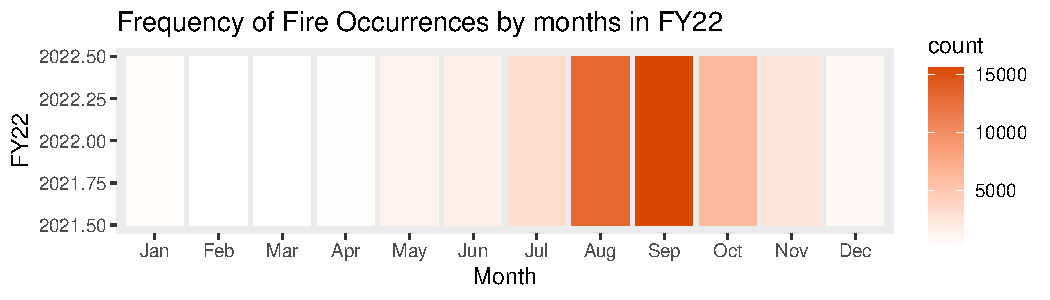
\includegraphics[width=\maxwidth]{figure/fire-by-months_fy22-1} \caption[Frequency of Fire Occurrences by months in FY22]{Frequency of Fire Occurrences by months in FY22}\label{fig:fire-by-months fy22}
\end{figure}

\end{knitrout}
\\From the table, we can clearly see that August and September are the riskiest months in terms of fire hazard, whereas November to July hardly pose any risk at all. It's natural to ask the follow-up question: How does FY22 compare to previous years? Is it valid to claim that August and September are the fire hazard season?



\begin{knitrout}
\definecolor{shadecolor}{rgb}{0.969, 0.969, 0.969}\color{fgcolor}\begin{kframe}
\begin{alltt}
\hlstd{heatmap_plot} \hlkwb{<-} \hlkwd{ggplot}\hlstd{(pivot_table,} \hlkwd{aes}\hlstd{(}\hlkwc{x} \hlstd{=} \hlkwd{factor}\hlstd{(abb_month,} \hlkwc{levels} \hlstd{= custom_order),}
                                        \hlkwc{y} \hlstd{=} \hlkwd{as.character}\hlstd{(year),} \hlkwc{fill} \hlstd{= count))} \hlopt{+}
  \hlkwd{geom_tile}\hlstd{()} \hlopt{+}
  \hlkwd{scale_fill_gradient}\hlstd{(}\hlkwc{low} \hlstd{=} \hlstr{"#fff7ec"}\hlstd{,} \hlkwc{high} \hlstd{=} \hlstr{"#d7301f"}\hlstd{)} \hlopt{+}
  \hlkwd{labs}\hlstd{(}\hlkwc{x} \hlstd{=} \hlstr{"Month"}\hlstd{,} \hlkwc{y} \hlstd{=} \hlstr{"FY13-22"}\hlstd{)} \hlopt{+}
  \hlkwd{theme_minimal}\hlstd{()} \hlopt{+}
  \hlkwd{theme}\hlstd{(}\hlkwc{axis.text} \hlstd{=} \hlkwd{element_text}\hlstd{(}\hlkwc{size} \hlstd{=} \hlnum{10}\hlstd{))}

\hlkwd{print}\hlstd{(heatmap_plot)}
\end{alltt}
\end{kframe}\begin{figure}
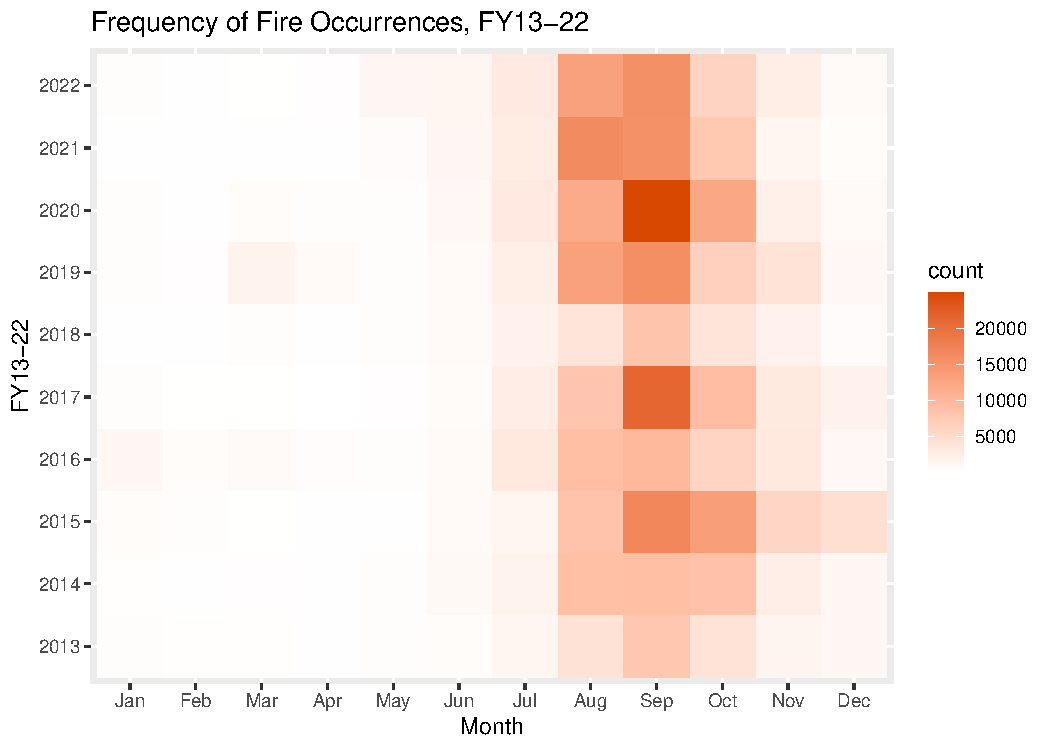
\includegraphics[width=\maxwidth]{figure/fire-by-months_fy13-22-1} \caption[Frequency of Fire Occurrences, FY13-22]{Frequency of Fire Occurrences, FY13-22}\label{fig:fire-by-months fy13-22}
\end{figure}

\end{knitrout}
\\Indeed, the data showed a trend indicating that August to October have more fire occurrences compared to the rest of the year. There are clearly more fire hazards in those months.
\\  
\\The foundation of a heatmap is a data matrix, where each entry in this matrix represents an observation or measurement. Therefore, the first step to create a heatmap is to organize the data by columns and rows. In Figure XXX, the structured data is displayed as a grid of coloured cells, where the colour intensity corresponds to the underlying frequency.
\\  
\\We have a one-to-one mapping of values to colours. The colour scale is mapped from the minimum to the maximum values. Colour scales can take the form of linear, logarithmic, or customed to enhance pattern visibility. The choice of the function depends on the context. In Figure Figure~\ref{fig:fire-by-months-fy13-22}, the frequency is linearly related to the colour scale. To use the logarithmic function would downplay the colour contrast. Therefore, in the case of visualizing fire occurrences, a linear scale preserves the contrast, faithfully representing the frequency.
\\  
\\Heatmaps are powerful tools for visualizing relationships between covariables within a model. One example of why we need to analyse a matrix of correlations between variables is in regression models. In the real world, variables are often correlated, and complete independent relations are rare. Consequently, analysing pairwise correlations is essential. Highly correlated variables significantly impact the regression model. When faced with highly correlated variables, we need to choose one variable from the correlated set. The selection is based on finding a regression model with the least Akaike Information Criterion (AIC) score among these variables. The AIC measures how much the linear model overfits the dataset. In other words, we want the regression model to explain the trend, and we do not want to overfit the model so that it explains the noise in the data set, which would lead to inaccurate predictions, as shown in Figure \ref{fig:noisy}.


\begin{figure}[h]
    \centering
    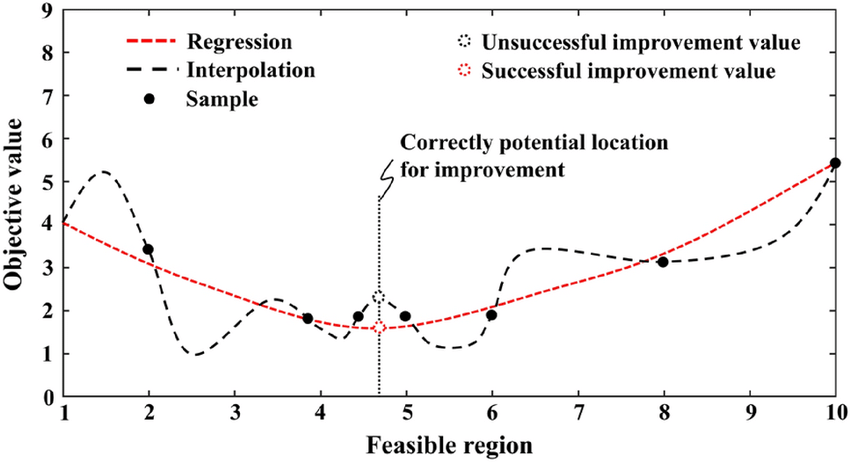
\includegraphics[width=0.7\textwidth]{/Users/margaretli/Data-Visualisation-Project/overfitting.png}
    \caption{Danger of overfitting the regression model}
    \label{fig:noisy}
\end{figure}




\subsection{3.4.2 Treemaps}
Treemaps are a visualisation method specifically designed for hierarchical data structures. They represent data as nested rectangles, where each rectangle represents a part of the whole. Treemaps offer a visually appealing and efficient way to convey the hierarchical composition of data. The size and color of each rectangle can be used to encode additional information.

\subsubsection{Use Cases for Treemaps}
Treemaps are highly effective when dealing with hierarchical data. Some common use cases include:
\begin{itemize}
\item \textbf{Disk Space Visualization}: Treemaps can be employed to visualize disk space usage, where the outermost rectangle represents the entire disk, and inner rectangles represent folders and files. The size of each rectangle reflects the space they occupy.
\item \textbf{Market Share Analysis}: In business, treemaps are useful for visualizing market share data. The top-level rectangle represents the total market, and inner rectangles represent individual segments, brands, or products. The size and color of each segment can represent its share and performance.
\end{itemize}

XXX %missing Treemaps


\section*{Chapter 3.5 Line Charts and Time Series Visualization}

A \textbf{Line chart}, often referred to as a line graph or line plot, is a statistical chart composed of a Cartesian coordinate system, some points, and lines. It is commonly used to represent changes in numerical values over continuous time intervals or ordered categories. In a line graph, the x-axis is typically used for continuous time intervals or ordered categories (such as Stage 1, Stage 2, Stage 3). The y-axis is used for quantified data, and if it is negative, it is plotted below the y-axis. Lines are used to connect adjacent data points.

Line graphs are used to analyze trends in things that change over time or ordered categories. If there are multiple sets of data, they are used to analyze the interaction and impact of these data sets over time or ordered categories. The direction of the line represents positive/negative changes, and the slope of the line indicates the degree of change.

In terms of data, a line graph requires a continuous time field or a categorical field and at least one continuous data field.


\subsection{Basic Components}
\begin{itemize}
  \item \textbf{X-Axis (Horizontal Axis):} Typically represents the independent variable, such as time or date.
  \item \textbf{Y-Axis (Vertical Axis):} Typically represents the dependent variable, like sales numbers, stock prices, or temperatures.
  \item \textbf{Line:} Connects the individual data points. In some line charts, multiple lines can represent different categories or sets of data.
\end{itemize}


\subsection{Suitability for Displaying Trends Over Time:}
\begin{itemize}
    \item \textbf{Visual Clarity:} Line charts provide a clear and concise way to view changes over time. When data points are plotted over regular intervals (e.g., days, months, years), it becomes easy to see upward or downward trends.
    \item \textbf{Comparisons:} When you have multiple lines on a single chart, you can easily compare different sets of data. For instance, comparing sales data of two different products over time.
    \item \textbf{Identification of Patterns:} Line charts help in identifying patterns and anomalies. Seasonal patterns, cyclical events, and unexpected spikes or dips become evident.
    \item \textbf{Forecasting:} By viewing historical data trends on a line chart, analysts can make predictions or forecasts for future data points.
    \item \textbf{Simplicity:} They are easy to understand and interpret. Even if someone isn't data-savvy, they can grasp the general trend and major fluctuations from a line chart.
    \item \textbf{Flexibility:} They can be used for both short-term and long-term data. Whether you're looking at stock prices minute-by-minute over a single day or global temperature averages over a century, line charts can effectively represent the data.
\end{itemize}


\subsection{Limitations:}
While line charts are excellent for displaying trends over time, they have limitations. They may not be suitable for showing individual data distributions or for data where there's no logical order. eg. too many points, too many lines, too many zeros.\\


\subsection*{Discuss the importance of time series visualisation in data analysis.}

Time series visualization refers to the graphical representation of time-ordered data points. In the world of data analysis, this form of visualization is invaluable for examining patterns, anomalies, and trends in datasets that evolve over time.\\
\textbf{Uncovering Trends:}\\
One of the primary advantages of time series visualization is the ease with which it allows analysts to identify long-term upward or downward trends in data. Recognizing these trends can help organizations make informed decisions about future strategies or interventions.\\
\textbf{Detection of Seasonality:}\\
Many datasets exhibit patterns that repeat over specific intervals, such as days, months, or years. Time series visualization makes it straightforward to spot such cyclical behaviors, which can be vital for businesses in sectors like retail or agriculture.\\
\textbf{Identifying Anomalies:}\\
Graphical representations can quickly highlight data points or periods that deviate significantly from the norm. These anomalies can indicate errors in data collection, or they may reveal significant events that need to be further investigated.\\
\textbf{Forecasting and Predictions:}\\
After identifying patterns in historical data, time series visualizations can aid in modeling future data points. Predictive modeling, underpinned by clear visualizations, allows businesses to make proactive decisions.\\
\textbf{Facilitating Comparative Analysis:}\\
Time series charts often allow for overlaying multiple data series on a single graph. This capability is useful for comparing different datasets or the same dataset under different conditions, leading to more comprehensive insights.\\
\textbf{Conclusion:}\\
Time series visualization is an indispensable tool in the arsenal of data analysts. It condenses large volumes of chronological data into easily interpretable graphics, enabling quick insights, better decision-making, and a deeper understanding of temporal dynamics in datasets. By providing a clear view of data trends, seasonality, and anomalies, time series visualization facilitates more informed and strategic actions in various domains.



\section*{Provide best practices for creating clear and informative line charts.}

\begin{itemize}
  \item Title and Labels: Every chart should have a descriptive title and axis labels to clearly convey the purpose of the visualization and the data being shown.
  \item Use of Colors: Colors should be chosen to clearly differentiate between different lines or data points but also be consistent with the overall theme or style.
  \item Gridlines and Background: Soft gridlines can help the viewer estimate values. A clean background aids in clarity.
  \item Line Types and Point Shapes: When multiple lines are on the same chart, use different line types and point shapes to differentiate between them.
  \item Consistent Scaling: The scale on the y-axis should be consistent so that the viewer isn't misled.
  \item Annotations: Important points or changes can be annotated directly on the graph.
  \item Legends: If there are multiple lines or data points with different colors/shapes, a legend should be provided.
\end{itemize}

Let's apply these practices:


First, we generate 2 series of random data.

\begin{knitrout}
\definecolor{shadecolor}{rgb}{0.969, 0.969, 0.969}\color{fgcolor}\begin{kframe}
\begin{alltt}
\hlstd{x} \hlkwb{<-} \hlkwd{seq}\hlstd{(}\hlnum{1}\hlstd{,} \hlnum{20}\hlstd{)}
\hlstd{y} \hlkwb{<-} \hlkwd{runif}\hlstd{(}\hlnum{20}\hlstd{)}
\hlstd{data} \hlkwb{<-} \hlkwd{data.frame}\hlstd{(}\hlkwc{x} \hlstd{= x,} \hlkwc{y} \hlstd{= y)}
\end{alltt}
\end{kframe}
\end{knitrout}

Below is a line chart of the random sample:

\begin{knitrout}
\definecolor{shadecolor}{rgb}{0.969, 0.969, 0.969}\color{fgcolor}
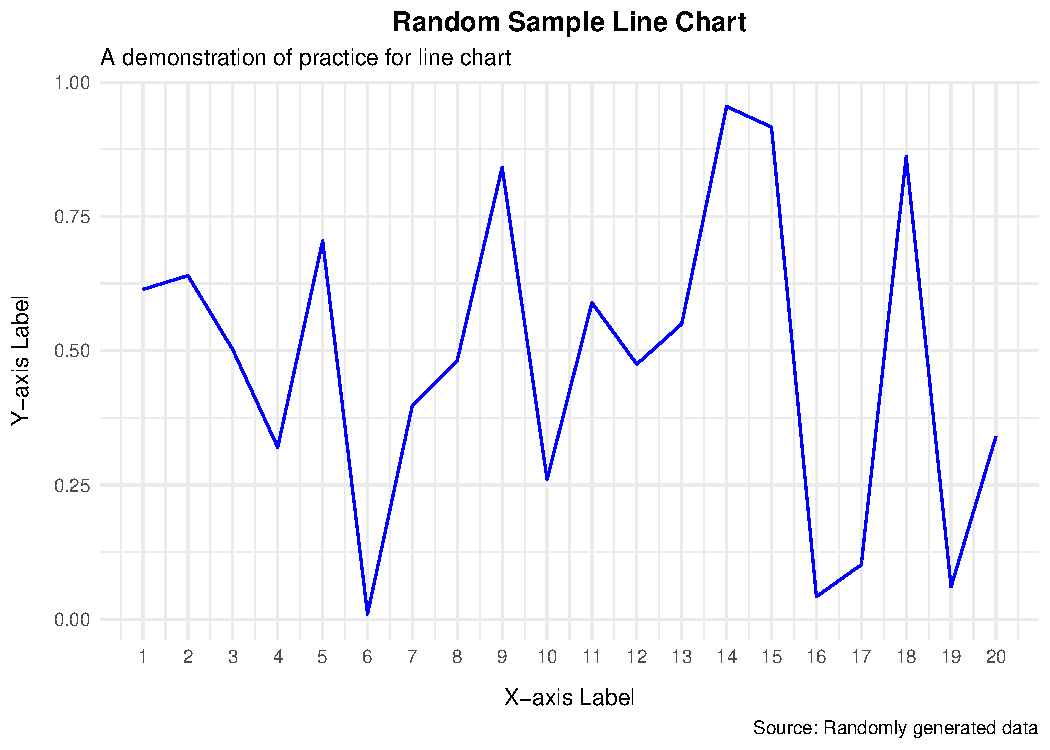
\includegraphics[width=\maxwidth]{figure/plot-chunk-1} 
\end{knitrout}


\section*{Showcase real-world examples of time series visualisations.}

Time series of the daily CNY, CAN, EUR, HKD, USD versus GBP exchange reference rate data
published by the European Central Bank over the time period from 01 Jan 2013 to 12 Oct 2023 (without weekends). The exchange rate tells you how many pounds you need to buy/sell 1 CNY, CAN, EUR, HKD, USD.

\subsection{The data set has the format as below:}

\begin{table}[h]
\centering
\begin{tabular}{|c|c|c|c|c|c|}
\hline
\textbf{Date} & \textbf{CNYtoGBP} & \textbf{CANtoGBP} & \textbf{EURtoGBP} & \textbf{HKDtoGBP} & \textbf{USDtoGBP} \\
\hline
\%d-\%m-\%y & Value & Value & Value & Value & Value \\
\hline
& & & & & \\
\hline
\end{tabular}
\caption{Field Information: CNY, CAN, EUR, HKD, USD to GBP}
\end{table}


\subsection{Multiple time series in one plot:}

\begin{knitrout}
\definecolor{shadecolor}{rgb}{0.969, 0.969, 0.969}\color{fgcolor}
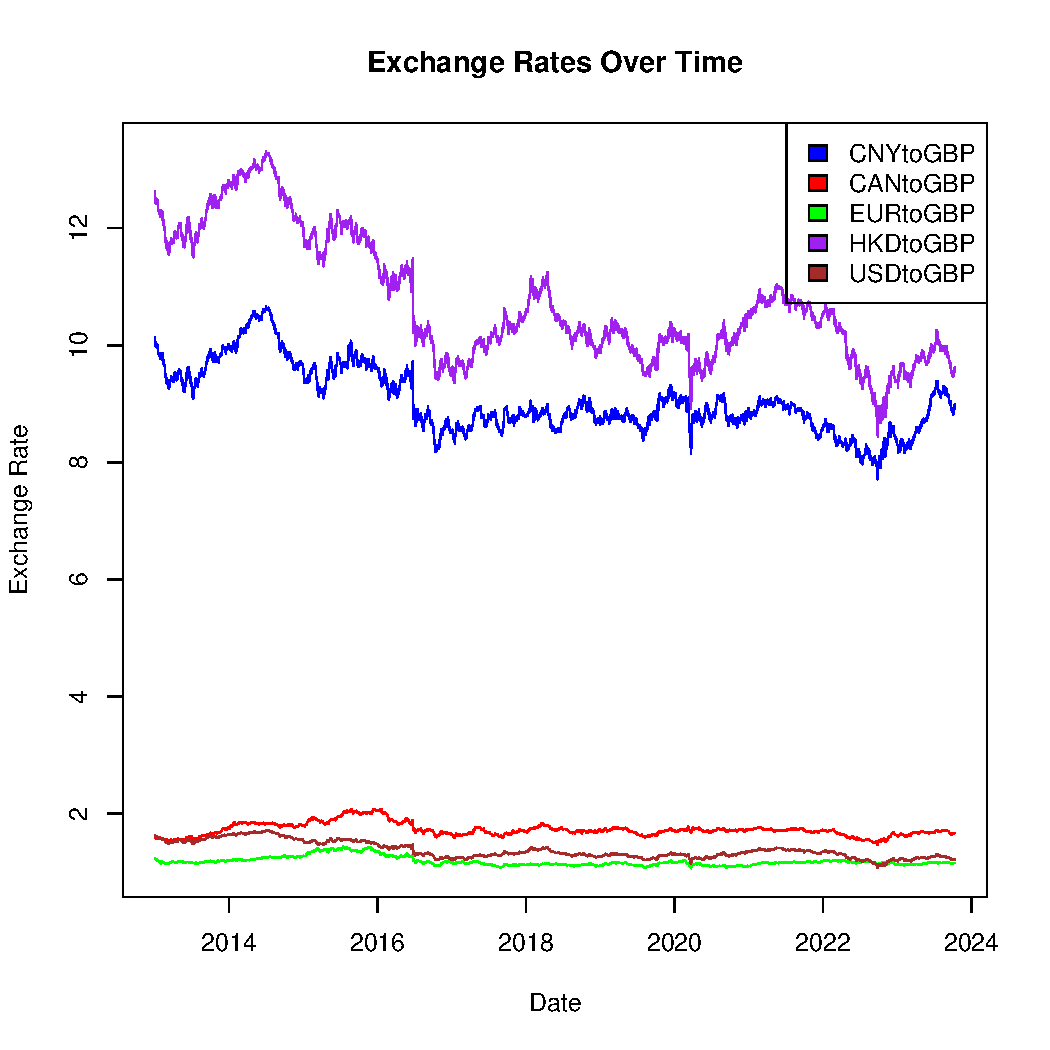
\includegraphics[width=\maxwidth]{figure/unnamed-chunk-1-1} 
\end{knitrout}

\subsection{Decomposition of one time series into trend, seasonal, and random.}


One of the primary advantages of time series visualization is the ease with which it allows analysts to identify long-term upward or downward trends in data and patterns that repeat over specific intervals. By decomposing the time series, it would be easy to see those features.

\begin{knitrout}
\definecolor{shadecolor}{rgb}{0.969, 0.969, 0.969}\color{fgcolor}
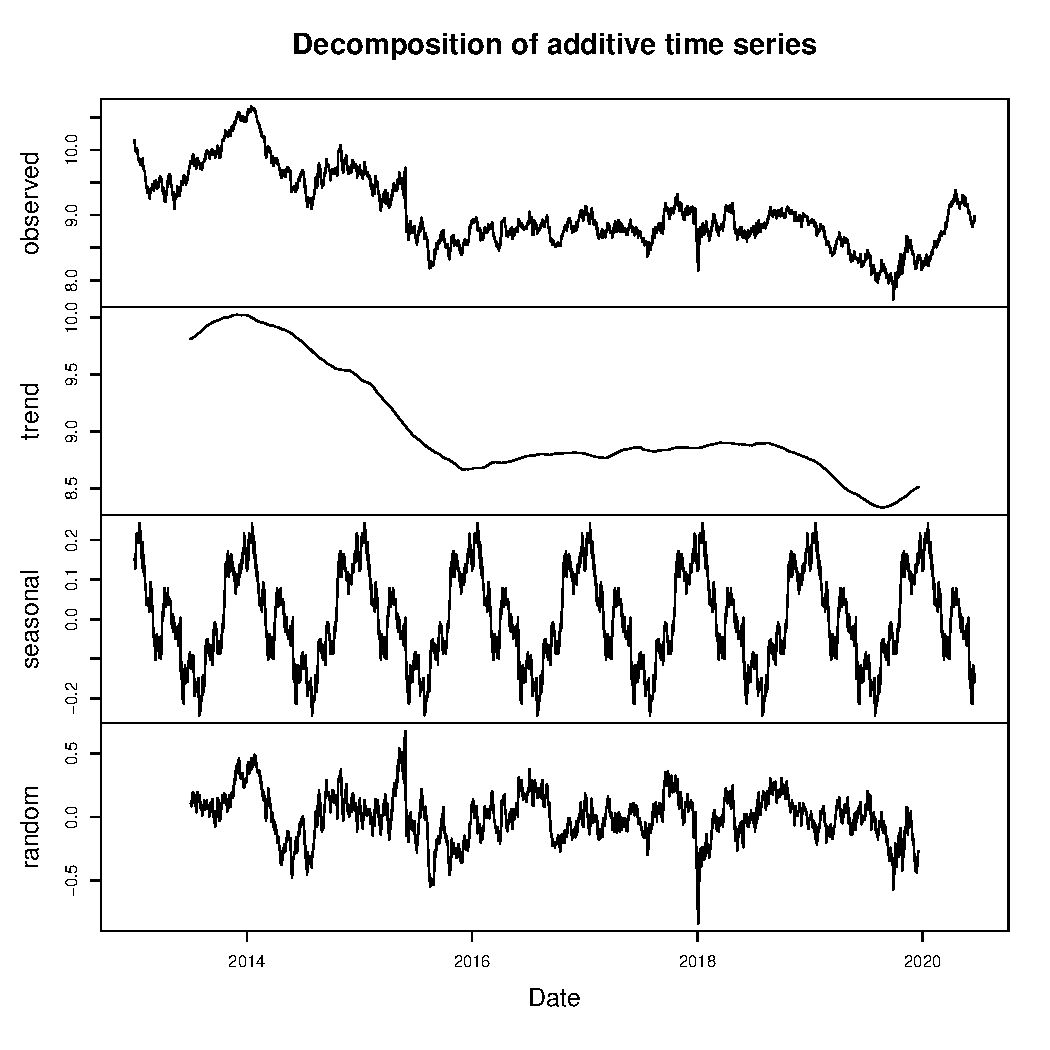
\includegraphics[width=\maxwidth]{figure/unnamed-chunk-2-1} 
\end{knitrout}


\subsection{Double y-axis time series plot.}

If we want to display two different time series that measure two different quantities at the same time points, we can draw the second series again on the second Y-axis on the right side.

\begin{knitrout}
\definecolor{shadecolor}{rgb}{0.969, 0.969, 0.969}\color{fgcolor}
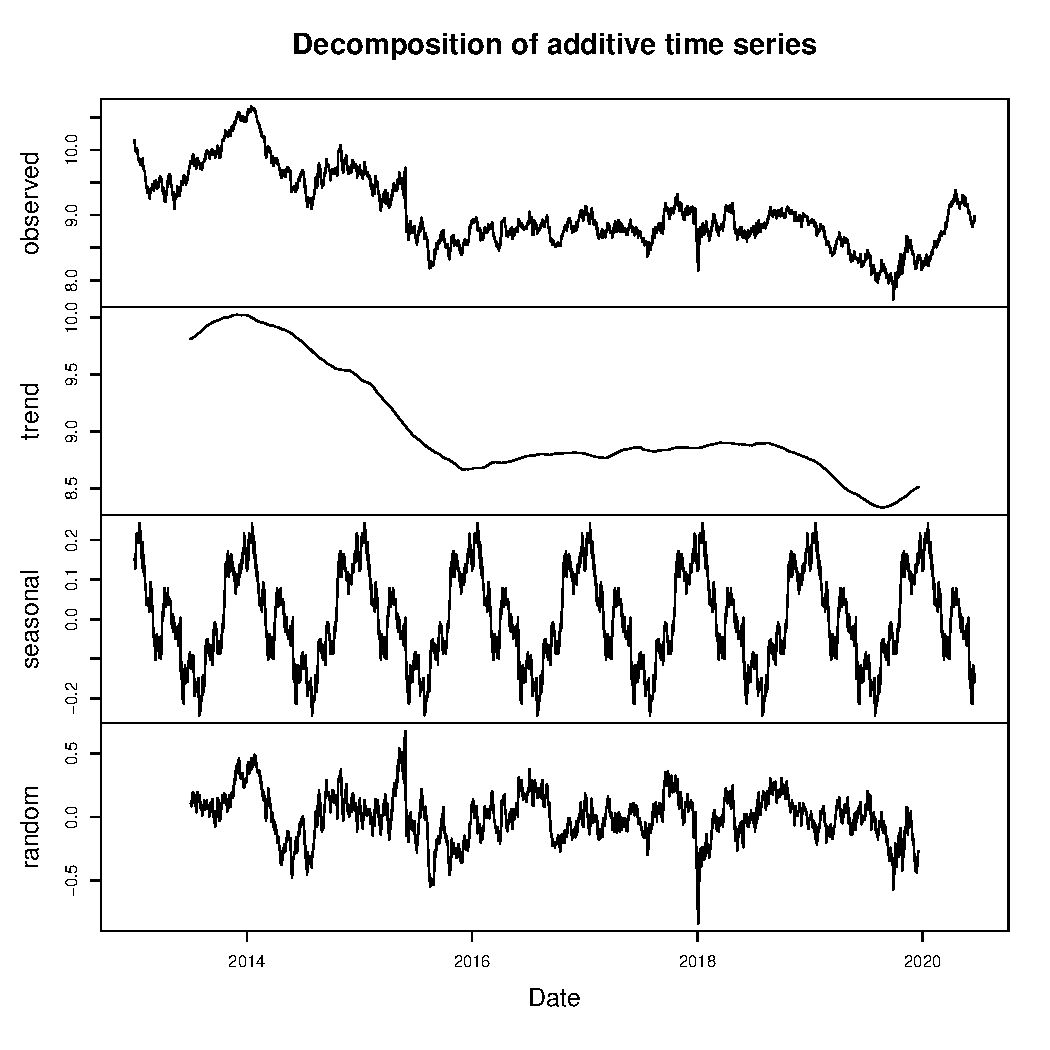
\includegraphics[width=\maxwidth]{figure/unnamed-chunk-3-1} 
\end{knitrout}


\section{Chapter 3.5 Network Graphs and Sankey Diagrams}
xxx

\section{Chapter 3.6 Geographic Maps and Spatial Data Visualisation}
xxx

\section{Chapter 3.7 3D and Interactive Visualisations}
xxx

\section{Chapter 3.8 Advanced Visualisation Techniques}
xxx


\end{document}
